\documentclass[12pt]{article}

\usepackage{algorithmic}
\usepackage{amsmath}
\usepackage{graphicx}
\usepackage{hyperref}
\usepackage{booktabs}

\providecommand{\e}[1]{\ensuremath{\times 10^{#1}}}

\begin{document}

\title{CSI709 Homework 5 \\
Fractional Power Filter}
\author{
        Geoffrey Ulman \\
        George Mason University\\
}
\date{\today}

\maketitle

\section{Results}

\begin{figure}
\centering
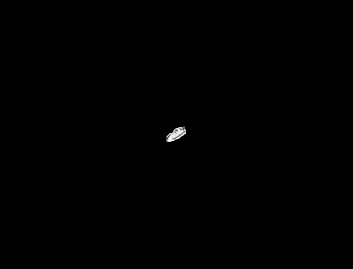
\includegraphics[width=0.50\textwidth]{plotBoat1.png}
\caption{Sample Boat Training Image 1}
\label{boats1}
\end{figure}

\begin{figure}
\centering
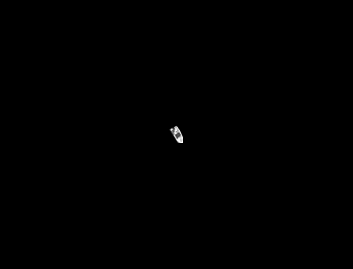
\includegraphics[width=0.50\textwidth]{plotBoat2.png}
\caption{Sample Boat Training Image 2}
\label{boats2}
\end{figure}

\begin{figure}
\centering
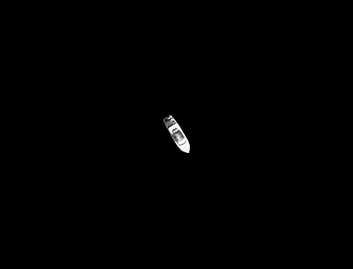
\includegraphics[width=0.50\textwidth]{plotBoat3.png}
\caption{Sample Boat Training Image 3}
\label{boats3}
\end{figure}

\begin{figure}
\centering
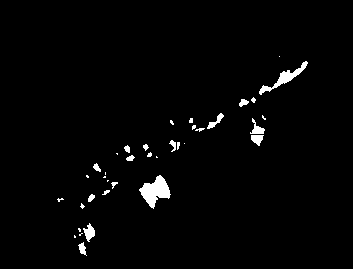
\includegraphics[width=0.50\textwidth]{boats_a00_peak1.png}
\caption{\(\alpha=0\) filtered peaks \(> 1.0\)}
\label{a00peak}
\end{figure}

\begin{figure}
\centering
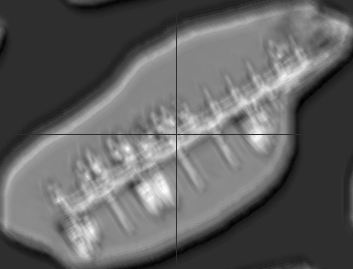
\includegraphics[width=0.50\textwidth]{boats_a00.png}
\caption{\(\alpha=0\)}
\label{a00}
\end{figure}

\begin{figure}
\centering
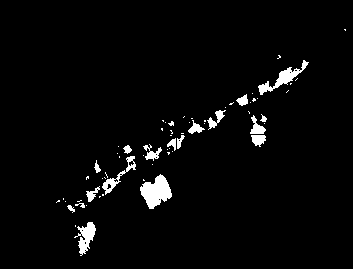
\includegraphics[width=0.50\textwidth]{boats_a04_peak9e-6.png}
\caption{\(\alpha=0.4\) filtered peaks \(> 9.0\e{-6}\)}
\label{a04peak}
\end{figure}

\begin{figure}
\centering
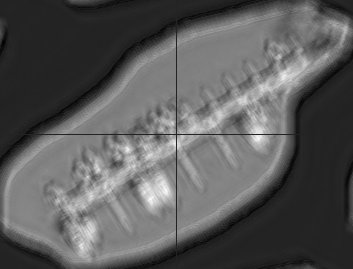
\includegraphics[width=0.50\textwidth]{boats_a04.png}
\caption{\(\alpha=0.4\)}
\label{a04}
\end{figure}

\begin{figure}
\centering
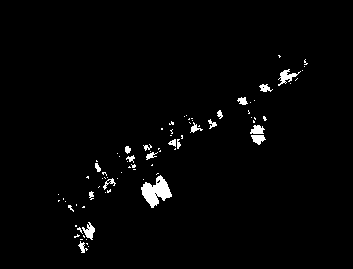
\includegraphics[width=0.50\textwidth]{boats_a08_peak9e-6.png}
\caption{\(\alpha=0.8\) filtered peaks \(> 9.0\e{-6}\)}
\label{a08peak}
\end{figure}

\begin{figure}
\centering
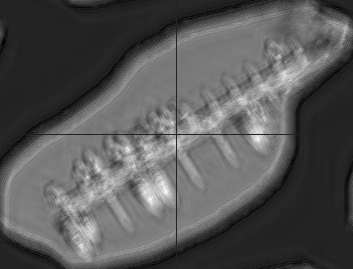
\includegraphics[width=0.50\textwidth]{boats_a08.png}
\caption{\(\alpha=0.8\)}
\label{a08}
\end{figure}

\begin{figure}
\centering
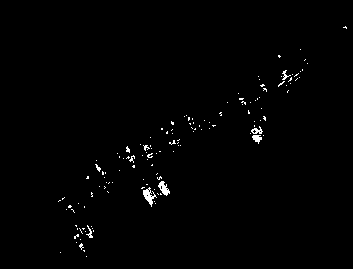
\includegraphics[width=0.50\textwidth]{boats_a12_peak7e-6.png}
\caption{\(\alpha=1.2\) filtered peaks \(> 7.0\e{-6}\)}
\label{a12peak}
\end{figure}

\begin{figure}
\centering
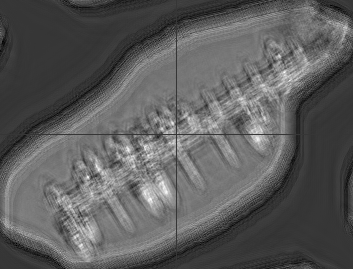
\includegraphics[width=0.50\textwidth]{boats_a12.png}
\caption{\(\alpha=1.2\)}
\label{a12}
\end{figure}

\begin{figure}
\centering
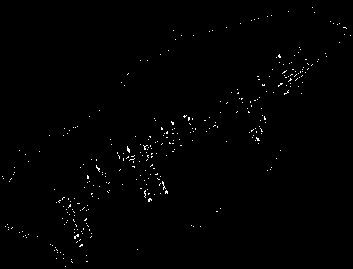
\includegraphics[width=0.50\textwidth]{boats_a16_peak5e-6.png}
\caption{\(\alpha=1.6\) filtered peaks \(> 5.0\e{-6}\)}
\label{a16peak}
\end{figure}

\begin{figure}
\centering
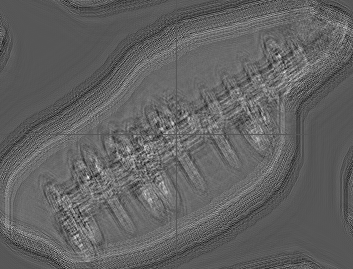
\includegraphics[width=0.50\textwidth]{boats_a16.png}
\caption{\(\alpha=1.6\)}
\label{a16}
\end{figure}

\begin{figure}
\centering
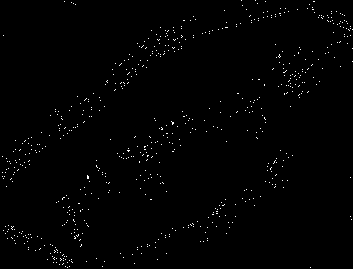
\includegraphics[width=0.50\textwidth]{boats_a20_peak5e-6.png}
\caption{\(\alpha=2.0\) filtered peaks \(> 5.0\e{-6}\)}
\label{a20peak}
\end{figure}

\begin{figure}
\centering
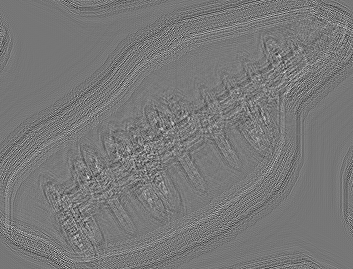
\includegraphics[width=0.50\textwidth]{boats_a20.png}
\caption{\(\alpha=2.0\)}
\label{a20}
\end{figure}

\end{document}
